\documentclass[1p]{elsarticle}

\usepackage{lineno,hyperref}
\modulolinenumbers[5]
\usepackage[utf8]{inputenc}
\usepackage[spanish]{babel}
\usepackage{amsmath}
\usepackage{todonotes}
\usepackage{listings}
\usepackage{graphicx}
\usepackage{amsfonts}
\usepackage[toc,page]{appendix}
\usepackage{amssymb}
\newtheorem{thm}{Teorema}
\newtheorem{lem}[thm]{Lema}
\newdefinition{rmk}{Remark}
\newproof{pf}{Demostración}
\newproof{pot}{Demostración del Teorema \ref{thm2}}
 
 \usepackage{listings}
 \usepackage{color}
 
 \definecolor{codegreen}{rgb}{0,0.6,0}
 \definecolor{codegray}{rgb}{0.5,0.5,0.5}
 \definecolor{codepurple}{rgb}{0.58,0,0.82}
 \definecolor{backcolour}{rgb}{0.95,0.95,0.92}
 
 \lstdefinestyle{mystyle}{
 	backgroundcolor=\color{backcolour},   
 	commentstyle=\color{codegreen},
 	keywordstyle=\color{magenta},
 	numberstyle=\tiny\color{white},
 	stringstyle=\color{codepurple},
 	basicstyle=\footnotesize,
 	breakatwhitespace=false,         
 	breaklines=true,                 
 	captionpos=b,                    
 	keepspaces=true,                 
 	numbers=left,                    
 	numbersep=5pt,                  
 	showspaces=false,                
 	showstringspaces=false,
 	showtabs=false,                  
 	tabsize=2
 }
 
 \lstset{style=mystyle}
%%\bibliographystyle{IEEEannot}

%% `Elsevier LaTeX' style
\bibliographystyle{elsarticle-num}
%%%%%%%%%%%%%%%%%%%%%%%
\usepackage{setspace}  
\begin{document}

\begin{frontmatter}

\title{A review of the paper: \textit{Inherent directionality explains the lack of feedback loops in
	empirical networks} }

%% Group authors per affiliation:
\author{Rubén Hurtado, Bartolomé Ortiz, Cristina Seva}
\address{Master en Física y Matemáticas\\ Universidad de Granada\\10/06/2018}

\begin{abstract}
This work is a brief revision and study about a paper called: \textbf{Inherent directionality explains the lack of feedback loops in empirical networks} written by \textit{Virginia Domínguez García, Simone Pigolotti and Miguel A. Muñoz}  . Our aim is to present its mains results, some technical highlights related to the mathematical and physical advances, and reproduce a minor result using our own methods. Its implications and future research will also be analysed. Although this work is merely a revision it could be useful as a source of code to reproduce some of the results.
\end{abstract}

\begin{keyword}
 \texttt{complex networks} \sep \texttt{mathematics}\sep \texttt{complexity} \sep \texttt{graph theory}
\end{keyword}

\end{frontmatter}
\setlength\parindent{0pt}
\linenumbers

\section{Introducción}
\spacing{1.5}
El objetivo de este trabajo es presentar el artículo seleccionado \cite{arti}, de manera que expondremos sus principales descubrimientos, así como algunas notas sobre los procedimientos que en él se presentan. 

Tras esto, vamos a realizar un pequeño intento de simulación para tratar de reproducir algunos de los resultados que aparecen en el articulo.

Finalmente, para cerrar nuestro trabajo, hablaremos un poco sobre las conclusiones obtenidas de este y sobre posibles vías para avanzar.

\section{Review del artículo}
\spacing{1.5}
El artículo muestra una serie de resultados que relacionan la direccionalidad inherente a muchos sistemas complejos empíricos (representados mediante grafos) con la ausencia de ciclos que se retroalimenten (\textit{feedback loops}) dentro de estos. 
Para empezar vamos a dar una pequeñas nociones sobre los elementos fundamentales del artículo:
\begin{itemize}
	\item \textbf{Direccionalidad inherente}: hablamos de direccionalidad inherente a un sistema complejo cuando, en el grafo que lo representa, todos los nodos se pueden ordenar en un eje unidimensional, de tal manera que los enlaces tienden a apuntar desde valores bajos a altos de sus coordenadas en dicho eje. 
	
	Como bien se apunta en \cite{arti}, la existencia de esta direccionalidad está relacionada con la existencia de una estructura jerárquica dentro de nuestra red. Así, aunque la aplicación de los resultados es muy amplia, podemos relacionarlo directamente con la temática de redes tróficas que vimos en clase. 

	\item \textbf{Ciclo retroalimentado o feedback loop}: hablamos de ciclo retroalimentado de orden $k$ dentro de un grafo direccional, cuando nos referimos una sucesión cerrada de $k$ nodos (esto es, con el mismo nodo en primera y última posición), cuyo orden de aparición viene determinado por el camino que indica el sentido de las aristas que los conectan.
        Por el contrario, llamamos \textbf{ciclo estructural} o simplemente ciclo de orden $k$ a un sucesión cerrada de nodos conectados en la que no se considera el sentido de las aristas.
\end{itemize}


    Debido al gran impacto de la existencia de feedback loops en la estabilidad dinámica del sistema, el artículo se centra en encontrar una herramienta predictiva para conocer  la fracción de ciclos para cada orden $k$ que también son ciclos retroalimentados, bajo el supuesto de que existe direccionalidad en la red caracterizada por un solo parámetro $\gamma$. 
    %Se observa, tanto experimentalmente como con la herramienta anterior, que esta fracción siempre es menor en redes con direccionalidad inherente que en redes aleatorizadas.

    El artículo se divide en tres puntos principales.
    En primer lugar, se diseña un modelo probabilístico para, bajo ciertas simplificaciones, obtener la probabilidad de que un ciclo de orden $k$ sea reatroalimentado en función de cierto parámetro $\gamma$ que indica la direccionalidad de la red.

    A continuación se analizan redes empíricas para obtener la fracción de ciclos retroalimentados frente a estructurales en estas.
    Se observa que esta fracción siempre es menor en redes con direccionalidad inherente que en redes aleatorizadas. 
    La excepción ocurre en redes socio-tecnológicas como la de los seguidores de Twitter, que analizaremos en datalle más adelante.
 
    
    Finalmente, se ajustan los datos experimentales usando dos métodos diferentes.
    Por una lado se obtiene el valor de $\gamma$ del modelo que mejor ajusta a los datos mediante mínimos cuadrados.
    Luego se ajustan los datos a una curva exponencial y se compara el resultado con la predicción asintótica del modelo, también exponencial, usando la $\gamma$ anteior.

    El buen ajuste que aparece en el artículo entre la predicción y los datos indica claramente la relación de causalidad entre la direccionalidad de la red y la ausencia de ciclos retroalimentados.


\subsection{Métodos}
    Exponemos ahora la forma de obtener la herramienta predictiva descrita en el artículo.

    Consideramos una red de $N$ nodos, y $L$ aristas.
    %e imaginamos que conocemos la fracción de ciclos retroalimentados de orden $k$: $F(k)$
     
    Asumimos que existe direccionalidad en esta red y la construimos aleatorizando la direccionalidad de la siguiente manera:
    para cada arista, con probabilidad $0<\gamma<1$ hacemos apuntar ésta en la dirección inherente, i.e.; hacia los nodos de mayor jerarquía, y con probabilidad $1-\gamma$ apunta en sentido contrario.
    Al parámetro $\gamma$ le llamaremos \textbf{parámetro de direccionalidad.}

    Dada esta red aleatoria, nos preguntamos, dado un valor de $\gamma$, cuál es la probabilidad de que un ciclo de orden $k$ se además retroalimentado. 
    Denotaremos esta probabilidad por $F(k, \gamma)$.

    Para ello, empezamos etiquetando con una notación jerárquica los nodos de este ciclo. 
    Existirán un total de $k!$ posibles ciclos estructurales, tantos como permutaciones de las etiquetas. 
    Para obtener la probabilidad buscada hemos de encontrar, de todos los ciclos anteriores, cuántos son retroalimentados.
    En general, la probabilidad de obtener un ciclo retroalimentado a partir de un ciclo cualquiera dependerá del número de ascensos $A(l,k)$.
    Este número cuenta cuántas permutaciones de la secuencia básica de longitud $k$ con $\textrm{nodo}_{i} < \textrm{nodo}_{i+1}$ se tienen para $l$ valores distintos de $i$. Para una secuencia no periódica, es decir, sin establecer ninguna relación entre el primer y último nodo, la solución a este problema está dada por los llamados \textbf{números eulerianos}.

    Sin embargo, como los ciclos que buscamos, al ser retroalimentados, están cerrados, se  generaliza el concepto de números de Euler para el caso periódico o cíclico.
    Es decir, necesitamos contar el número de ascensos en un ciclo cerrado genérico, lo que en el articulo se bautiza como los \textbf{numeros eulerianos cíclicos}, denotados por $A(l,k)$.
Con este interesante concepto en mente, los autores ya pueden desarrollar la expresión de la función buscada: %necesitando ahora añadirle el parametro de direccionalidad:
    \begin{equation}
    \label{eq:F_exact}
        F(k,\gamma)=\sum_{l=0}^{k}\frac{A(l,k)}{k!}[\gamma^l(1-\gamma)^{k-l}+\gamma^{k-l}(1-\gamma)^l]
    .
    \end{equation}
Aquí se multiplica el número de permutaciones con $l$ ascensos, $A(l,k)$, por su probalidad de ocurrencia, que aparece en el corchete.
Ésta se obtiene trivialmente a partir de $\gamma$ que corresponde a la probabilidad de ascenso. Finalmente, se divide el resultado por el número total de permutaciones $k!$ para obtener la fracción de ciclos retroalimentados.

Usando los procesos del material suplementario, esta expresión puede aproximarse, en el caso de $k$ grande y $\gamma$ no muy pequeño, por:
\begin{equation}
    \label{eq:F_asymp}
    F(k,\gamma)
    \approx 
    2\exp\left\{\frac{k}{2}\log[\gamma(1-\gamma)]+\frac{k}{24} \log^2(\frac{\gamma}{1-\gamma})\right\}
\end{equation}

    Este proceso nos permite obtener una expresión teórica con la que comparar los datos experimentales, con los que se ajusta además muy bien.
    Sin embargo, no hay que perder de vista que en la obtención de la ecuación~\ref{eq:F_exact} se ha hecho una simplifación importante: cada ciclo se ha considerado de forma completamente independiente;
    se han obviado posibles relaciones entre ciclos o diferencias entre éstos a diferentes alturas de la estructura jerárquica.
    En el análisis del artículo esto no supone ningún problema, lo que justifica como válidas las aproximaciones anteriores.
    Sin embargo, en nuestro intento de reproducción sí jugarán un papel muy importante.

%Esta expresión es la que hemos usado para todas las partes replicadas de nuestra revisión. \todo{seguro?}
    Para concluir, presentamos en la gráfica \ref{h}, que también se puede ver en \cite{arti}, la relación entre el parámetro de forma $\gamma$ y la fracción $F(k,\gamma)$.

\begin{figure}
	\centering
	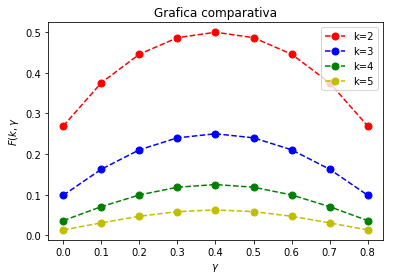
\includegraphics[width=12cm]{graf_1.png}
	\caption{$F(k)$ frente a $\gamma$, se puede observar el pico en $\gamma=1/2$}
	\label{h}
\end{figure}



\subsection{Algunos resultados a destacar}
Entrando en la parte de resultados, queremos destacar algunos de los que nos han parecido más relevantes.
\begin{itemize}
	\item La fracción de los ciclos de retroalimentación de cualquier longitud $k$ es mucho más pequeña en redes biológicas y ecológicas de lo que cabría esperar para cualquier otro grafo similar pero aleatorizado.
	\item El número total de ciclos de retroalimentación también se reduce 
	con respecto a las aleatorizaciones de red. Sin embargo, y esto es por lo que nos llamó la atención realizarlo en Twitter, estas tendencias no son tan evidentes para las redes socio-tecnológicas; mientras que todas las redes consideradas tienen una fracción más pequeña de bucles de retroalimentación que sus aleatorizaciones de direccionalidad, la red social de Twitter exhibe una mayor $F(k)$ que las aleatorizaciones.
	\item Por supuesto, el modelo desarrollado reproduce bastante bien las muestras experimentales obtenidas, que muestran un decaimiento exponencial de $F(k)$ conforme aumenta $k$.
        Esto puede observarse desde dos perspectivas.
        Por un lado, las $X$ en el gráfico representan la predicción del modelo cuando $\gamma$ ha sido ajusta mediante mínimos cuadrados a los datos.
        Aquí podemos ver que en la amplia mayoría de los casos hay un muy buen acuerdo entre los valores experimentales y el modelo.
        Por otro lado, se compara la predicción asintótica del modelo de la ecuación \ref{eq:F_asymp} con una regresión exponencial a los datos.
        Aquí de nuevo observamos una muy buena coincidencia.
        
\end{itemize}

Para observar gráficamente estos resultados podemos irnos a la gráfica \ref{h1}, donde hemos destacado la sección de redes tecnológicas. Antes, no obstante, debemos hacer una reseña sobre la información a encontrar:

 En la gráfica se compara la fracción medida de los ciclos retroalimentados $F(k)$ con dos aleatorizaciones de la misma red. La primera, que llaman aleatorización de la direccionalidad (DR) - conserva las aristas existentes, pero aleatoriza completamente sus direcciones. La segunda, aleatorización de configuración (CR), aleatoriza tanto aristas como direcciones, pero preservando la conectividad de entrada y salida de cada nodo.
\begin{figure}
	\centering
	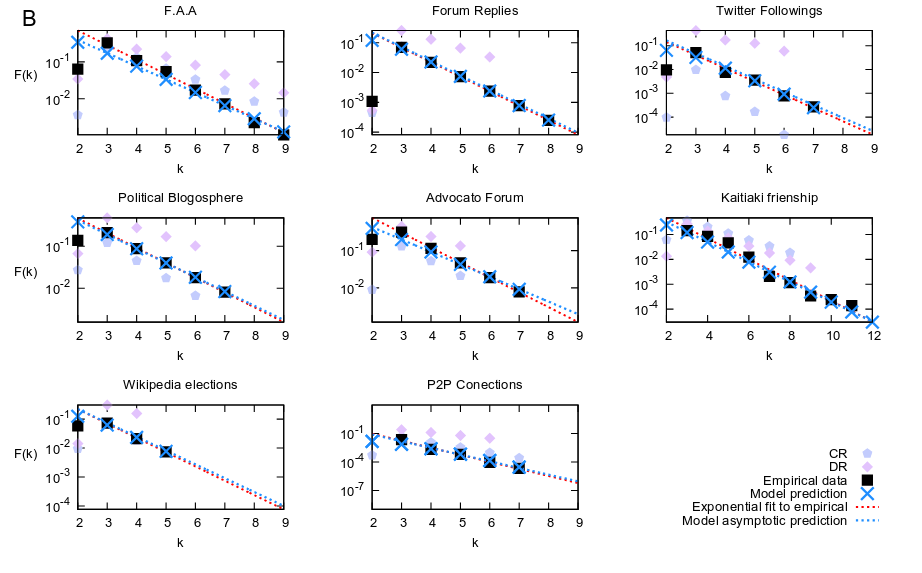
\includegraphics[width=15cm]{graf_2.png}
	\caption{Gráfico extraído del artículo donde resaltamos la parte de redes tecnológicas}
	\label{h1}
\end{figure}

Finalmente queremos resaltar el apartado sobre cómo disponer de información sobre nuevos nodos puede alterar lo que sabemos hasta ahora por las predicciones.

 Para probar la robustez
de su predicción, los investigadores simularon el efecto de desconocimiento sobre las redes que ya tenían,
eliminando una fracción de los enlaces al azar, y repitieron el análisis anterior. 

Aunque esta operación afecta claramente a la cantidad de enlaces, las conclusiones del modelo apenas varían, lo cual nos parece muy interesante. Incluso cuando la cifra de nodos que se elimina está entre $20\%$ y $50\%$ es posible observar esta tendencia en la gráfica obtenida del material suplementario \ref{h4}
\begin{figure}
	\centering
	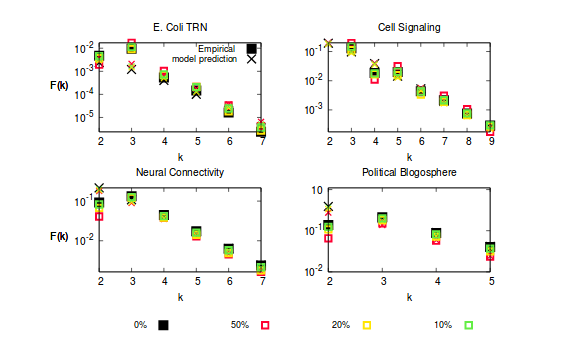
\includegraphics[width=15cm]{graf_3.png}
	\caption{Gráfico extraído del artículo donde resaltamos el impacto de los nodos o conexiones no observadas}
	\label{h4}
\end{figure}

\section{Intento de reproducción}
\spacing{1.5}

Desde el principio nos atrajo la cantidad de aplicaciones que la investigación podía tener, por eso decidimos escoger este artículo para el trabajo. Durante su lectura acordamos que la mejor manera de intentar comprenderlo era la reproducción parcial de los resultados y, con tal fin, pensamos que debíamos escoger alguna red a la que tuviéramos fácil acceso.

Pasó por nuestra cabeza la posibilidad de fijarnos en las redes tecnológicas que se exponían al final, pues contenían detalles interesantes como hemos descrito antes.

En particular, nos centramos en la reproducción de redes en Twitter. 
%En este caso estaríamos ante una predicción como la que se observa en la gráfica \ref{h2}.
%\todo{es coherente con el resto?}
%\begin{figure}
%	\centering
%	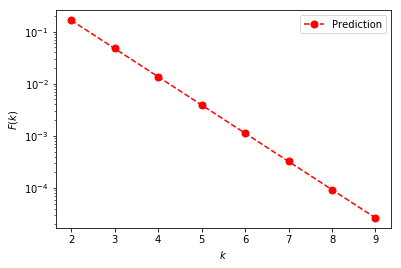
\includegraphics[width=9cm]{graf_4.png}
%	\caption{Gráfico extraído del artículo donde resaltamos la parte de redes tecnológicas}
%	\label{h2}
%\end{figure}

\subsection{Metodología}
\spacing{1.5}
    Una vez elegida la red pasamos a su estudio.
    Éste se dividió en dar partes: primero buscamos un conjunto de datos sobre los que trabajar y luego se procedió a su análisis.
    
    En la primera, inicialmente nos basamos en la base de datos expuesta en el material complementario de \cite{arti}. 
    Lamentablemente, el volumen de los datos echaba por tierra cualquier intento por nuestra parte, debido a la poca capacidad computacional de nuestros ordenadores.

Estando en esta situación, decidimos que la mejor manera de sobreponernos era obtener nuestra propia fuente de datos, de una de nuestras redes (más pequeña que la usada en el estudio) de Twitter.

    Para ello usamos el paquete \textit{Tweepy}, el cual nos ofrece la posibilidad de conectarnos a la API de twitter para la obtención de nuestro grafo de seguidores.
    Hemos de destacar que las restricciones de petición de usuarios a la aplicación hicieron que nos retrasásemos, pues nuestro dataset tardó días en estar completo.
    Éste se generó partiendo de la red de seguidores/seguidos de uno de los miembros del grupo y ampliándola con las redes de 50 de sus seguidores, elegidos aleatoriamente.
    Con este proceso, obtuvimos un grafo dirigido con 40375 nodos y 41480 aristas.

    Una vez completo el dataset, pasamos a analizar la información mediante el paquete \textit{NetworkX}:
	 En primer lugar, obtuvimos los ciclos estructurales de nuestra red. Para ello utilizamos una versión no-recursiva de iterador/generador del algoritmo de Johnson, implementada por nosotros basada en la librería de NetworkX, definida como:
\begin{lstlisting}[language=Python]
    def simple_cycles_undirected(G, maxlength=float('inf'))
\end{lstlisting}
    Este algoritmo parte de un nodo y viaja la red usando una búsqueda en profundidad (\textit{Depth First Search}) para hallar ciclos. Esta búsqueda termina cuando se recorre toda la región accesible desde el nodo de partida o se alcanza una profundidad máxima especificada, tras lo que se repite el proceso con otro nodo hasta utilizarlos todos.

    Aquí nos volvimos a topar con la velocidad de ejecución.
    Aun siendo el algoritmo elegido bastante bueno en cuanto a complejidad y tiempo de ejecución, nuestros ordenadores no eran lo suficientemente rápidos lo que nos hizo perder mucho tiempo en obtener resultados.

    Luego utilizamos otra función implementada en la librería de NetworkX para el conteo de ciclos de retroalimentación en grafos dirigidos, definida como :

\begin{lstlisting}[language=Python]
    feedback_cycle_list_DG1 = (list(simple_cycles(DG1)))
\end{lstlisting}

    Una vez obtenida la información sobre la ditribución de nodos en nuestra red, pasamos a repetir el análisis del artículo 

    Como extra, puede consultar el código de nuestro workflow en el apéndice.


\subsection{Resultados}

\begin{figure}
    \centering
    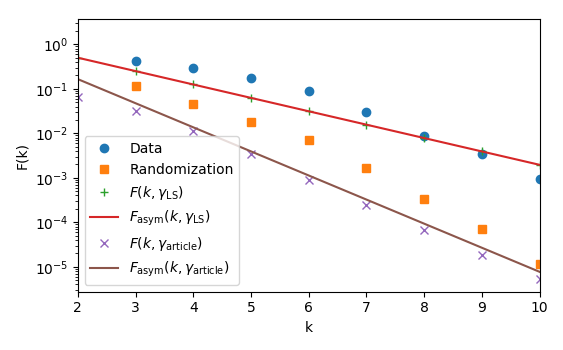
\includegraphics[width=0.5\paperwidth]{F_sevaseviene.png}
    \caption{Fracción de los ciclos estructurales en nuestra red de Twitter que también son retroalimentados, $F(k)$, frente a su orden (cículos azules). También se muestra los valores $F(k)$ correspondientes para red aleatorizada (círculos naranjas). Junto a a estos datos se muestra la predicción del modelo $F(k, \gamma)$ para la $\gamma$ que mejor ajusta a los datos por mínimos cuadrados, $\gamma_{LS}$ (cruces verdes), y la correspondiente a la del artículo $\gamma_{article}$ (equis moradas). También se muestran las predicciones asintóticas del modelo para estas dos $\gamma$ (línea roja y línea marrón, respectivamente).}
    \label{fig:sevaseviene_F}
\end{figure}

    Los resultados obtenidos según el proceso anterior se muestran en la figura~\ref{fig:sevaseviene_F}.
    En ésta se muestran los valores experimentales obtenidos de $F(k)$ para nuestra red de Twitter. 
    Podemos ver que, al igual que en el artículo, nuestra red presenta una $F(k)$ mayor al caso aleatorizado, en contraste con lo que ocurre en redes ecológicas y biológicas. 
    El valor de $F(k)$ para la aleatorización corresponde al método DR y es el resultado de promediar sobre 1000 aleatoriazaciones.

    Sin embargo, al contrario que en el artículo, ajustando $\gamma$ al modelo mediante mínimos cuadrados obtenemos $\gamma_{LS} \simeq 0.50$, que coincide muy mal con los datos.
    Esto implica que la distribución de ciclos de nuestra red no puede ser explicada mediante el modelo propuesto.

    Comparando con los resultados con el $\gamma$ obtenido en el artículo, $\gamma_{\textrm{article}} = 0.967$, vemos que tampoco hay un buen ajuste, aunque la pendente para ordenes mayores parece coincidir con la de nuestros datos.

\begin{figure}
    \centering
    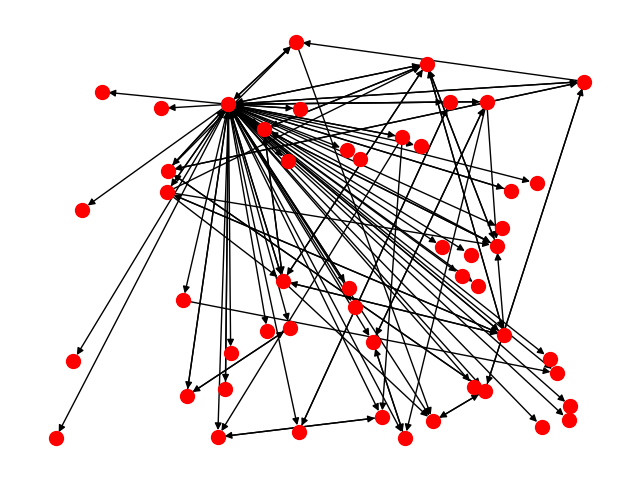
\includegraphics[width=0.5\paperwidth]{graph_sevaseviene.png}
    \caption{Representación de los nodos con grado de salida mayor que 0 en nuestra red.}
    \label{fig:sevaseviene_network}
\end{figure}

    Estos resultados puede explicarse por nuestra muestra de la red de Twitter.
    Al haber sido generada a partir de la red de un usuario, esta se muestra completamente sesgada a éste.
    Esto puede observarse claramente en la figura~\ref{fig:sevaseviene_network}, en la que están representados los nodos de nuestra red con orden de salida y de entrada mayor que cero, es decir, aquellos que pueden contribuir a ciclos.
    
    Debido a este sesgo, la mayoría de ciclos contienen a este usuario: 228745 sobre 229062 en el caso de ciclos estructurales y 1052 sobre 1110 en el caso de los retroalimentados.
    Esta circunstancia incumple claramente la suposición del modelo de que los ciclos sean independientes, lo que justifica el poco acierto del modelo en nuestra reproducción.

    A pesar de esto, la coincidencia de la pendiente para $k$ grande al usar la forma asintótica de $F(k, \gamma)$ con $\gamma_{\textrm{article}}$ parece indicar que, aunque de forma más compleja, la direccionalidad de la red sigue estando presente.

    Por otra parte, podemos intentar explicar la abundancia de ciclos con respecto a la red aleatorizada, presente tanto en nuestros datos como en el artículo.
    En Twitter, además de una clara direccionalidad hacia los usuarios más famosos, similar a lo que ocurre en redes tróficas, existe un gran número de conexiones bidireccionales entre usuarios a un mismo nivel. Estas relaciones, que no existen de forma tan marcada en redes biológicas, serían las causantes del aumento de $F(k)$.


\section{Conclusiones finales}
\spacing{1.5}
    Para finalizar, remarcamos algunas de puntos más importantes de nuestro intento de reproducción.

    En primer lugar, nos ha llamado la atención la gran necesidad de potencia computacional para resolver el problema. 
    Conceptos aparentemente sencillos como los de ciclos estructurales o dirigidos se convierten en problemas tremendamente costosos a nivel computacional, que hacen irrealizables el análisis de redes relativamente grandes.

    Por otra parte hemos visto que la red de Twitter, desde un punto de vista local, no satisface el modelo propuesto del artículo. Sin embargo, la coincidencia de las pendientes en el gráfico de $F(k)$ parece indicar que la direccionalidad de la red también es observable desde esta perspectiva, sólo que requeriría de correciones para tener en cuenta la no independencia de los diferentes ciclos.

    Finalmente, una dirección interesante en la que avanzar sería el estudio de la red de Twitter analizando de forma conjunta tanto su carácter direccional como la asortatividad en las conexiones recíprocas.

\section*{Referencias}
\spacing{1.5}
\bibliography{bibliograf}

\begin{appendices}
	
	\section{Workflow de conversión y resultados}
	\lstinputlisting[language=Python]{../workflow.py}
\pagebreak
\section{Obtención de datos en twitter}
\lstinputlisting[language=Python]{../follow.py}
\end{appendices}



\end{document}
